\chapter{ANN Architectures for Njets2 and Njets3 Categories}
\label{app:nns_architecture}

\begin{figure}[H!]{16cm}
	\vspace{-20cm}
	\caption{The architecture of the neural network created in this analysis for \textbf{Njets2} category. The black dots represent the inputs and the neurons, while the lines represent the size of the parameters found after training those NNs. Wider and brighter lines means that the parameter (weight or bias) associated to a given input for a neuron is larger (in other words its contribution is more relevant). This ANN has 21:13:8 hidden neurons of SeLU type.}
	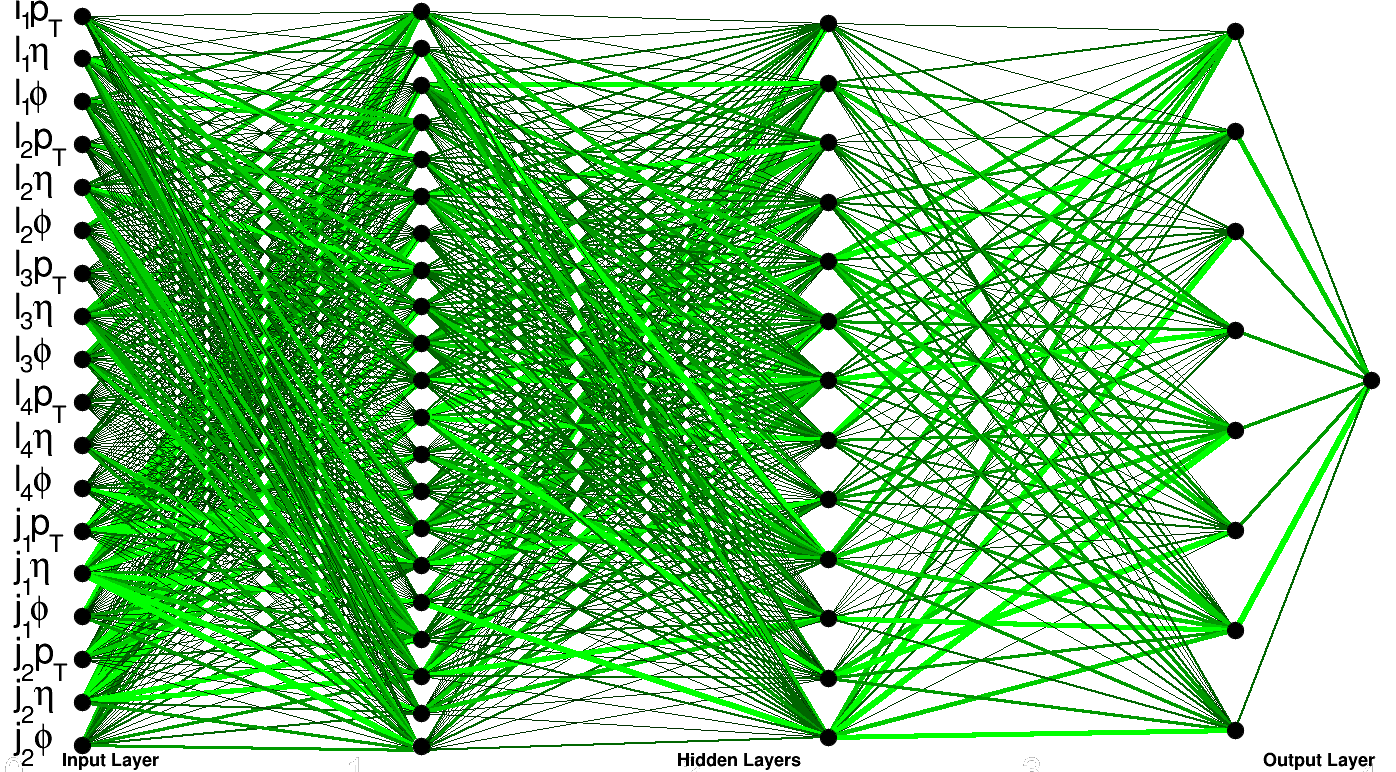
\includegraphics[width=18cm,height=11cm,angle=90]{ChapterAnalysis/figs/k57nj2_architecture_horizontal}
	\source{The AUTHOR, 2018.}
\end{figure}
	
\begin{figure}[H!]{16cm}
	\caption{The architecture of the neural network created in this analysis for \textbf{Njets3} category. This ANN has 11:9:7 hidden neurons of SeLU type.}
	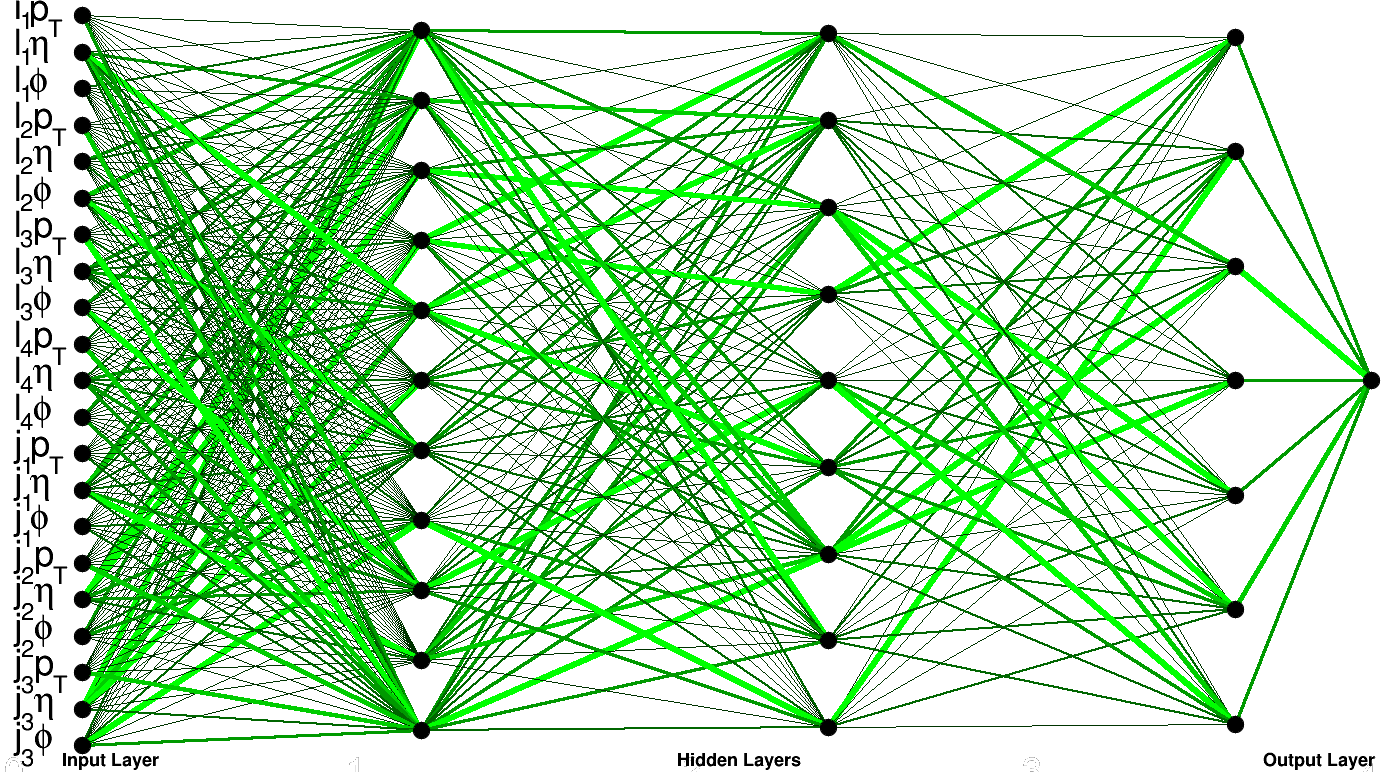
\includegraphics[width=18cm,height=11cm,angle=90]{ChapterAnalysis/figs/k24nj3_architecture_horizontal}
	\source{The AUTHOR, 2018.}
\end{figure}

\chapter{Expected $S/\sqrt{B}$ and $\pi~.~S/(S+B)$ Combining Njets2 and Njets3 Cuts}
\label{app:significance_cutting_NNs}

\begin{figure}[H!]{16cm}
	\vspace{-20cm}
	\caption{The significance (computed as $S/\sqrt{B}$) (a) and the efficiency times purity ($\pi.\epsilon$) (b) achieved when cutting at the NN for each jet-based category. The cut applied corresponds to the low edge value of a given bin in the histogram. Note that the significance computed here does not take into account the uncertainties.}
	\subfloat[]{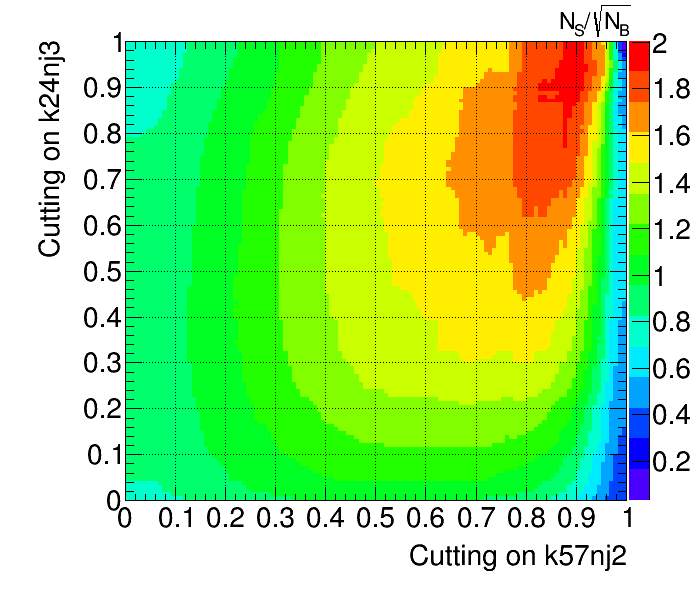
\includegraphics[width=10cm,height=8cm]{ChapterAnalysis/figs/Significance_versus_NNs_cutting}}\\
	\subfloat[]{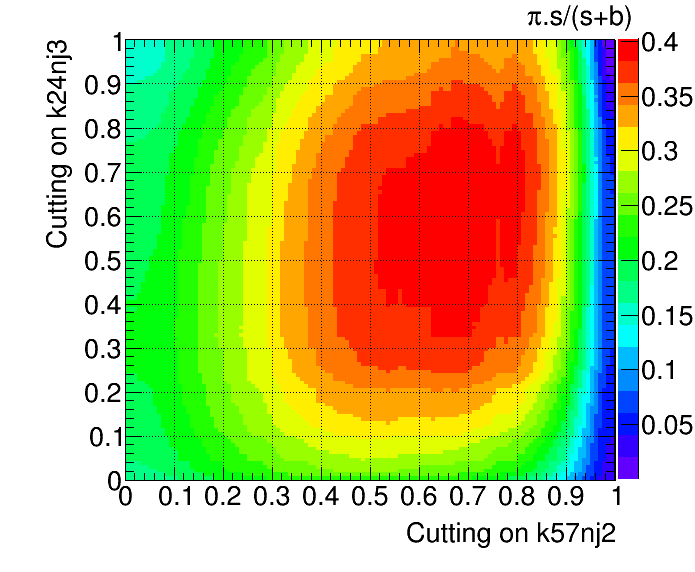
\includegraphics[width=10cm,height=8cm]{ChapterAnalysis/figs/EfficiencyTimesPurity_versus_NNs_cutting}}
	\source{The AUTHOR, 2018.}
\end{figure}

		
%\section{Datacard from Njets2 and Njets3 Categories Combination \label{app:combination_datacard}}
%\begin{center}
%	
\includegraphics[scale=0.7,angle=-90,trim={3cm 28cm 165cm 3cm},clip]{figs/combinedCard_Higgs125GeV_VBFStudy_k57nj2_k24nj3_4l}\\
%	
\includegraphics[scale=0.7,angle=-90,trim={35cm 28cm 131.5cm 8cm},clip]{figs/combinedCard_Higgs125GeV_VBFStudy_k57nj2_k24nj3_4l}\\
%	
\includegraphics[scale=0.7,angle=-90,trim={67cm 28cm 99cm 8cm},clip]{figs/combinedCard_Higgs125GeV_VBFStudy_k57nj2_k24nj3_4l}\\
%	
\includegraphics[scale=0.7,angle=-90,trim={101cm 28cm 64cm 8cm},clip]{figs/combinedCard_Higgs125GeV_VBFStudy_k57nj2_k24nj3_4l}\\
%	
\includegraphics[scale=0.7,angle=-90,trim={135.7cm 28cm 10cm 8cm},clip]{figs/combinedCard_Higgs125GeV_VBFStudy_k57nj2_k24nj3_4l}\\	
%\end{center}
